\section{Cosmological analyses with the \lya\ forest power spectrum}
\label{sec:over}

In this section we present an overview of the different aspects involved in 
a cosmological analysis of the small scale clustering from the \lya\ forest
power spectrum.

\begin{itemize}
 \item Measurement of the flux power spectrum: calibrate the quasar spectra, 
  fit the quasar continua, measure 2-point functions, covariance matrices 
  and possible contaminants.
 \item Infer the linear power spectrum: using hydrodynamical simulations, 
  build an emulator to translate the measured flux power to constraints 
  on the linear power spectrum of density at the redshift of the measurement
  ($z \sim 3$).
 \item Cosmological constraints: combine the inferred linear power spectrum
  with external datasets (primarily CMB studies) to constraint the parameters
  of a particular cosmological model.
\end{itemize}


\subsection{Measuring the \lya\ correlations}

Skip over continuuming fitting, instrumental details, and so on.
This will not be the main focus of this paper.

In most cases, the line of sight wavenumbers are expressed in units of 
inverse velocity, $\ikms$, but other mappings from observed wavelength 
could be used.
When measuring the 3D power, we will also need to define transverse 
wavenumbers, and in this case the natural choice is to use units of 
inverse angles \cite{Font-Ribera2018}.

\begin{figure}[h]
 \begin{center}
  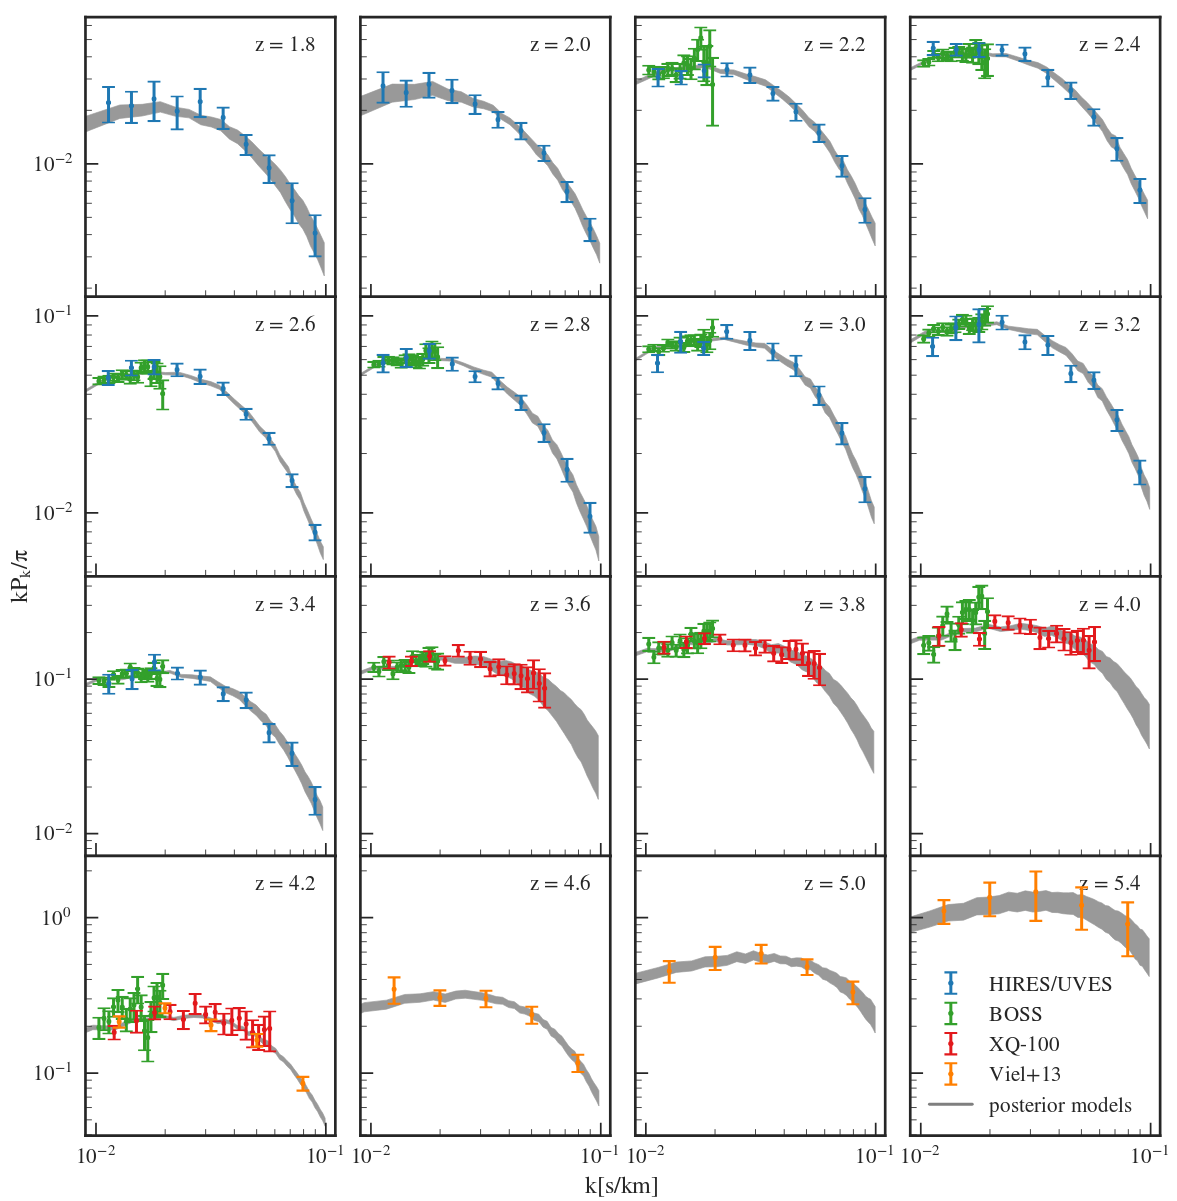
\includegraphics[scale=0.4]{Figures/Walther2018_P1D}
  %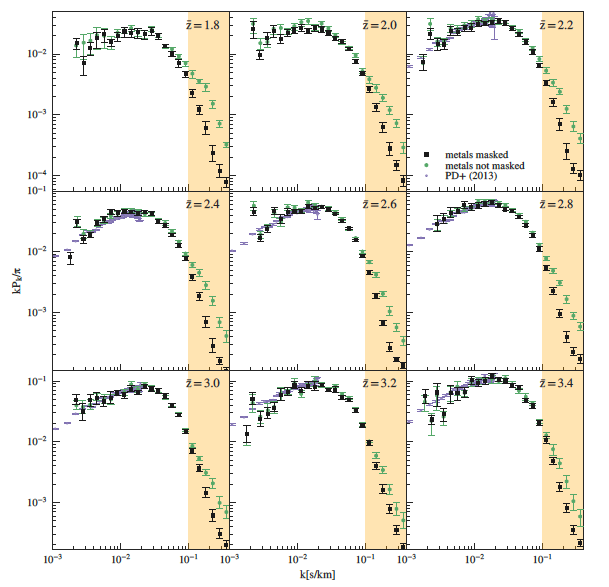
\includegraphics[scale=0.6]{Figures/WaltherP1D}
 \end{center}
 \caption{Compilation of $P_{1D}(z,\kpar)$ measurements, including those from
  \cite{Viel2013} (orange), \cite{Irsic2017} (red), 
  \cite{Palanque-Delabrouille2013} (green) and \cite{Walther2018} (blue). 
  This figure was stolen from \cite{Walther2018}.
 }
 \label{fig:dataP1D}
\end{figure}

Beyond BAO analyses \cite{Bautista2017,duMasdesBourboux2017}, the only 
public results on the clustering of the \lya\ forest are measurements of 
the 1D power spectrum \cite{Croft1998,McDonald2000,McDonald2006} or 
more recently \cite{Viel2013,Palanque-Delabrouille2013,Irsic2017,Walther2018}.
These are usually presented as band powers measured in different redshift
bins, spanning the redshift $1.8 < z < 5.4$, and covering a broad range of 
scales $0.001 \ikms < \kpar < 0.1 \ikms$. 
A compilation of recent measurements is shown in Figure \ref{fig:dataP1D}.


\subsection{Infering the linear power spectrum}

This step is the main one discussed in this paper.

\AFR{Add here a discussion on the main difficulties in building an emulator,
include discussion on hydro simulations, box size, resolution, the nuisance
of modelling thermal history, mean flux, but also rescaling of optical depth.}

Add a first, brid

\subsection{Cosmological constraints}

Discuss how the flux power mostly measures amplitude and slope around k=1, and 
it is only in combination with CMB that one can break degeneracies and 
constraint multiple cosmological parameters, including neutrino mass. 

\AFR{Mention that some studies have merged the last two steps
\cite{Palanque-Delabrouille2015,Yeche2017}, and argue why we think this 
might not be a good idea.}

